\documentclass[main.tex]{subfile}
\begin{document}
    \section{Embedded}
    \subsection{Microcontroller}
    \subsection{Custom Software}
    \subsection{Buses}
    \subsection{Main Embedded Board}
    Raspberry Pi’s will be socketed on the main embedded board face down (as described by the CAD). Due to the complexity of the board, and minimal space saved by integrating the board onto the main embedded system, the Pi will not be integrated directly onto the main embedded. Furthermore, in case of a malfunction it is more cost and time effective to replace a singular Pi instead of replacing the entire board. The Arduino Mega will be integrated directly onto the board. Since once complete the Arduinos will not have to be frequently updated, it would be efficient to simply use a ATmega 328, DIP-28 package and pop it out to program it on a regular Mega board when necessary. The choice for a DIP package over a TQFP was also made such that a blown chip would not lead to the entire board having to be replaced.

    \subsection{Subsystem Boards}
    Originally, the embedded team decided to use an Arduino Uno, with a CANBUS shield stacked on top, with a seperate board with the connections to the external connectors on it. However, most of the pins on both the arduino and the CANBUS were completely unnecessary. With said design, the embedded for a single subsystem would be almost triple the size of an Arduino Uno, with significantly more sources of error (the Arduino, the CANBUS, and a board housing connectors would have to be connected together).  Upon considering that there would have to be multiple of these housings, it was decided that all three boards could be integrated into a singular one, with the approximate size of an Arduino Uno. Once the final revision is designed, multiple copies of the same board will be printed and populated. For initially testing purposes however the original setup of an Uno with a CANBUS shield will be used, until the PCB is printed and thoroughly tested.

    \subsection{Sensors}
    \subsubsection{Temperature}
    \subsubsection{Current}
    \subsubsection{Tilt}
    \subsubsection{Navigation}
    \subsubsection{Lateral Stability}
    \subsubsection{EC-Brake State}
    \subsubsection{Pressure}

    \subsection{Thermal}
    \subsection{Flowcharts}

    \subsection{Physical Hardware}
    Mass, power, etc.\\
    How will these things be powered? Mini lipo battery packs?\\
    How is it mounted? CAD? Does it need to be in a pressure chamber?\\
    Will the processors get very hot due to vacuum? How will they be cooled?\\
    Will the system have components susceptible to vacuum? (e.g. some capacitors) Briefly justify an answer of “no.” How will we test this?\\
    Rationale for choosing Raspberry Pi and Arduino\\
    Cost breakdown

    \subsection{Software System Structure}
    \subsubsection{Terminology}
    \begin{itemize}
        \item Control-Panel - UI interface running on a remote machine to visualize data and control pod
        \item Master Machine - RaspberryPi 3B computer running Waterloop’s communication-system
        \item Slave Machine - Arduino Due running Waterloop’s embedded-system
        \item CAN Data Packet - Custom binary packet type created by team Waterloop
    \end{itemize}
    \subsubsection{Design Criteria}
    The main goal  when building the software systems around the pod was creating a redundant, yet lightweight and fast solution that would allow for safe communications with the vehicle and ensure control throughout pod launch. The Software-system is built upon the Master-Slave design model to allow for maximum redundancy and safety at all times. The design is based on three components: embedded systems (Slave), communication systems (Master), and control-panel. Embedded-systems is responsible for all of the pod’s internal interactions with the sensors and various health checks. Communication-systems is responsible for the complete pod control and has the ability to safely shut down the pod in case of an emergency. It is also responsible for the transportation of information from the vehicle to the front-end to allow for live data visualization and remote control of the pod. Front-end is responsible for displaying all of the pod’s vital readings and providing an interface to control the pod while in the tube. All of the code written for the software system of the pod is available for public access at Waterloop’s github page.
    \subsubsection{System Overview}
    Building off the model of Master-Slave design, Waterloop has defined two clear computational layers Master Machines and Slave Machines. Master machines are responsible for the complete control of the pod and the transfer of data from Slave Machines to the Control-Panel. Two main design decisions of the Goose III’s computational design are the parallelism of launch script execution and the Master-slave design.
    \begin{itemize}
        \item Having Master-Slave design in place, we can ensure the validity of data coming from the Slave Machines. When Slaves acquire data from sensors, there is a possibility of a slave providing errant data. To handle the case of an errant slave, Masters have the voting capability to compare the results of three slaves, detect the errant device and act appropriately
        \item With parallel execution by the two Master machines, in case of one of the machines coming offline for any unforeseen reason, the switch to the next machine is instantaneous
    \end{itemize}
    \textbf{[INSERT SOFTWARE DIAGRAM HERE]}\\
    Based on the software diagram above, the entire system will incorporate \textbf{[Number of sensors]} sensors and an ESC, that will allow for a complete control over the pod and a live stream of data from all sensors.
    \subsubsection{Control Packet Format}
    \paragraph{JSON}
    All communications between onboard computers and frontend controls are JSON packets serialized from Go structs in the following format:
    \begin{verbatim}
type CommPacketJson struct {
    Time int64     `json:"time"`
    Type string    `json:"type"`
    Name string    `json:"name"`
    Data []float32 `json:"data"`
}
    \end{verbatim}
    \begin{table}[H]
        \centering
        \begin{tabular}{@{}lll@{}} \toprule
            Property & Description & Example\\ \midrule
            \verb|time| & Time of packet creation, in milliseconds since Unix epoch & \verb|1513452619442|\\
            \verb|type| & Packet type, see possible packet types & \verb|"sensor"|\\
            \verb|name| & \makecell[l]{Specific name of packet, explicitly describing role and origin of packet \\ (i.e. data from a specific sensor)} & \verb|"accel1"|\\
            \verb|data| & 3-tuple of float32 values representing packet data & \verb|[32.2323, 12.22, 23.11]|\\ \bottomrule
        \end{tabular}
        \caption{Explanation of fields}
    \end{table}
    Example of a serialized JSON:
    \begin{verbatim}
{
    "time": 1513452619442,
    "type": "sensor",
    "name": "accel",
    "data": [0.00, 0.00, 0.00]
}
    \end{verbatim}
    \subsubsection{Communication Protocol}
    Commands, sensor data, and events are sent between data machines, controllers, and web servers, using 64-bit packets. Packets are memory-		efficient, fast to read and write, and reliable. Packets are checked with a CRC-8 checksum $(0$x$97 = x^8 + x^5 + x^3 + x^2 + 1)$.
    \begin{table}[H]
    	\centering
    	\begin{tabular}{@{}lccccc@{}} \toprule
            Segment & Type & Sensor ID & Data 1 & Data 2 & Data 3 \\ \midrule
            Bits & 3 & 7 & 18 & 18 & 18 \\ \bottomrule
        \end{tabular}
        \caption{Caption here}
    \end{table}
    Each packet contains 3 bits representing packet type, 7 bits representing origin sensor or device ID, and three 18-bit data segments. These are 18-bit floats with 1 bit for sign, 5-bit exponent width, and 13-bit significand precision (12 explicitly stored), similar to IEEE 754 specifications.
	\begin{figure}[H]
        \centering
        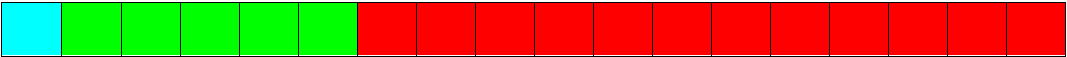
\includegraphics[width = \textwidth]{images/fig326}
    	\caption{Caption here}
    \end{figure}
    \subsection{Navigation System}
    \subsection{Library \& Build Infrastructure}
    We developed an in-house C++ library for use on microcontrollers (Arduino and Raspberry Pi). WLib is performant, memory efficient, has a small binary footprint, and is a safer alternative to STL. WLib uses a custom memory management solution with fixed-size memory pools, preventing fragmentation and leaks. It provides basic data structures (lists, sets, maps, trees), and smart pointers (shared and unique).
    \url{https://teamwaterloop.github.io/waterloop-wlib/}

    We also developed a custom Arduino build system and use Cosa, an object-oriented AVR platform, in place of the standard Arduino libraries. Cosa (\url{https://github.com/mikaelpatel/Cosa}) is faster and has lower power consumption.
    \subsection{Fault Tolerance \& Testing}
    \subsection{Pod Health}
\end{document}
